% Chapter 3: Methodology
% Required packages in main document: graphicx, float, geometry, setspace, hyperref

\chapter{Methodology}

\section{Introduction}

This chapter presents the methodology adopted in the design and development of the automated pinhole detection system for banknote paper quality control. The system integrates embedded hardware, computer vision, machine learning, and wireless communication technologies to achieve reliable and automated detection of pinholes in paper. The methodology covers the overall system architecture, the working principle of pinhole detection, the hardware components selected and their individual roles, the software design, and the mechanical structure of the system.

\section{System Architecture}

The system is composed of two main subsystems: a hardware detection unit and a software processing unit, which communicate over a Wi-Fi network.

The hardware detection unit consists of an ESP32 microcontroller, an ESP32-CAM module, a bright light source, Light Dependent Resistors (LDRs), a wiper motor, a relay module, a buck converter, a 12V power supply, and a 20$\times$4 I\textsuperscript{2}C LCD display. The wiper motor drives the paper through the detection chamber, where the bright light shines through the paper from one side while LDR sensors on the opposite side measure transmitted light intensity to detect pinholes.

The ESP32-CAM captures images of the paper under inspection and transmits them to the software unit via an HTTP API route over Wi-Fi. The software unit, running on a host computer, receives the images, processes them through a trained machine learning model built with Python, and returns detection results. The software communicates commands back to the detection hardware using the MQTT protocol, enabling real-time closed-loop control of the system.

\section{Working Principle of Pinhole Detection}

The fundamental principle behind the system is light transmission through pinholes. During normal operation, the bright light source illuminates one side of the banknote paper while the paper travels through the detection chamber driven by the wiper motor. Under a defect-free section of paper, the paper absorbs or scatters most of the light, resulting in a low reading at the LDR sensors on the opposite side.

When a pinhole is present in the paper, light passes directly through the hole and reaches the LDR sensors on the other side with a measurably higher intensity. This increase in detected light intensity triggers a detection event. The LDR readings are continuously monitored by the ESP32, which simultaneously operates the ESP32-CAM to capture an image of the suspect region. The image is then forwarded to the software system for further classification and confirmation via the trained machine learning model.

This dual approach — combining real-time LDR-based light sensing with image-based machine learning classification — ensures both speed and accuracy in pinhole detection.

\section{Hardware Components}

The following subsections describe each hardware component used in the system, its specifications, and its specific role in the detection process.

\subsection{Light Dependent Resistors (LDRs)}

\begin{figure}[H]
    \centering
    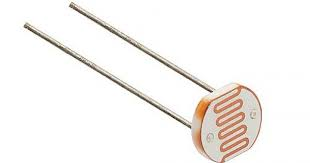
\includegraphics[width=0.4\textwidth]{pictures/LDR.jpg}
    \caption{Light Dependent Resistor (LDR)}
    \label{fig:ldr}
\end{figure}

A Light Dependent Resistor (LDR), also known as a photoresistor, is a passive electronic component whose electrical resistance decreases as the intensity of incident light increases. As shown in Figure~\ref{fig:ldr}, the LDR is a compact, disc-shaped component with a characteristic serpentine conductive track on its surface.

In this system, LDRs are positioned on the side of the paper opposite to the bright light source. During normal scanning, the paper blocks most of the light and the LDRs register a high resistance (low voltage output). When light passes through a pinhole, the resistance of the corresponding LDR drops sharply, producing an elevated voltage that the ESP32 detects as an anomaly. Multiple LDRs are arranged across the width of the paper to provide full coverage of the inspection area.

\subsection{Bright Light Source}

\begin{figure}[H]
    \centering
    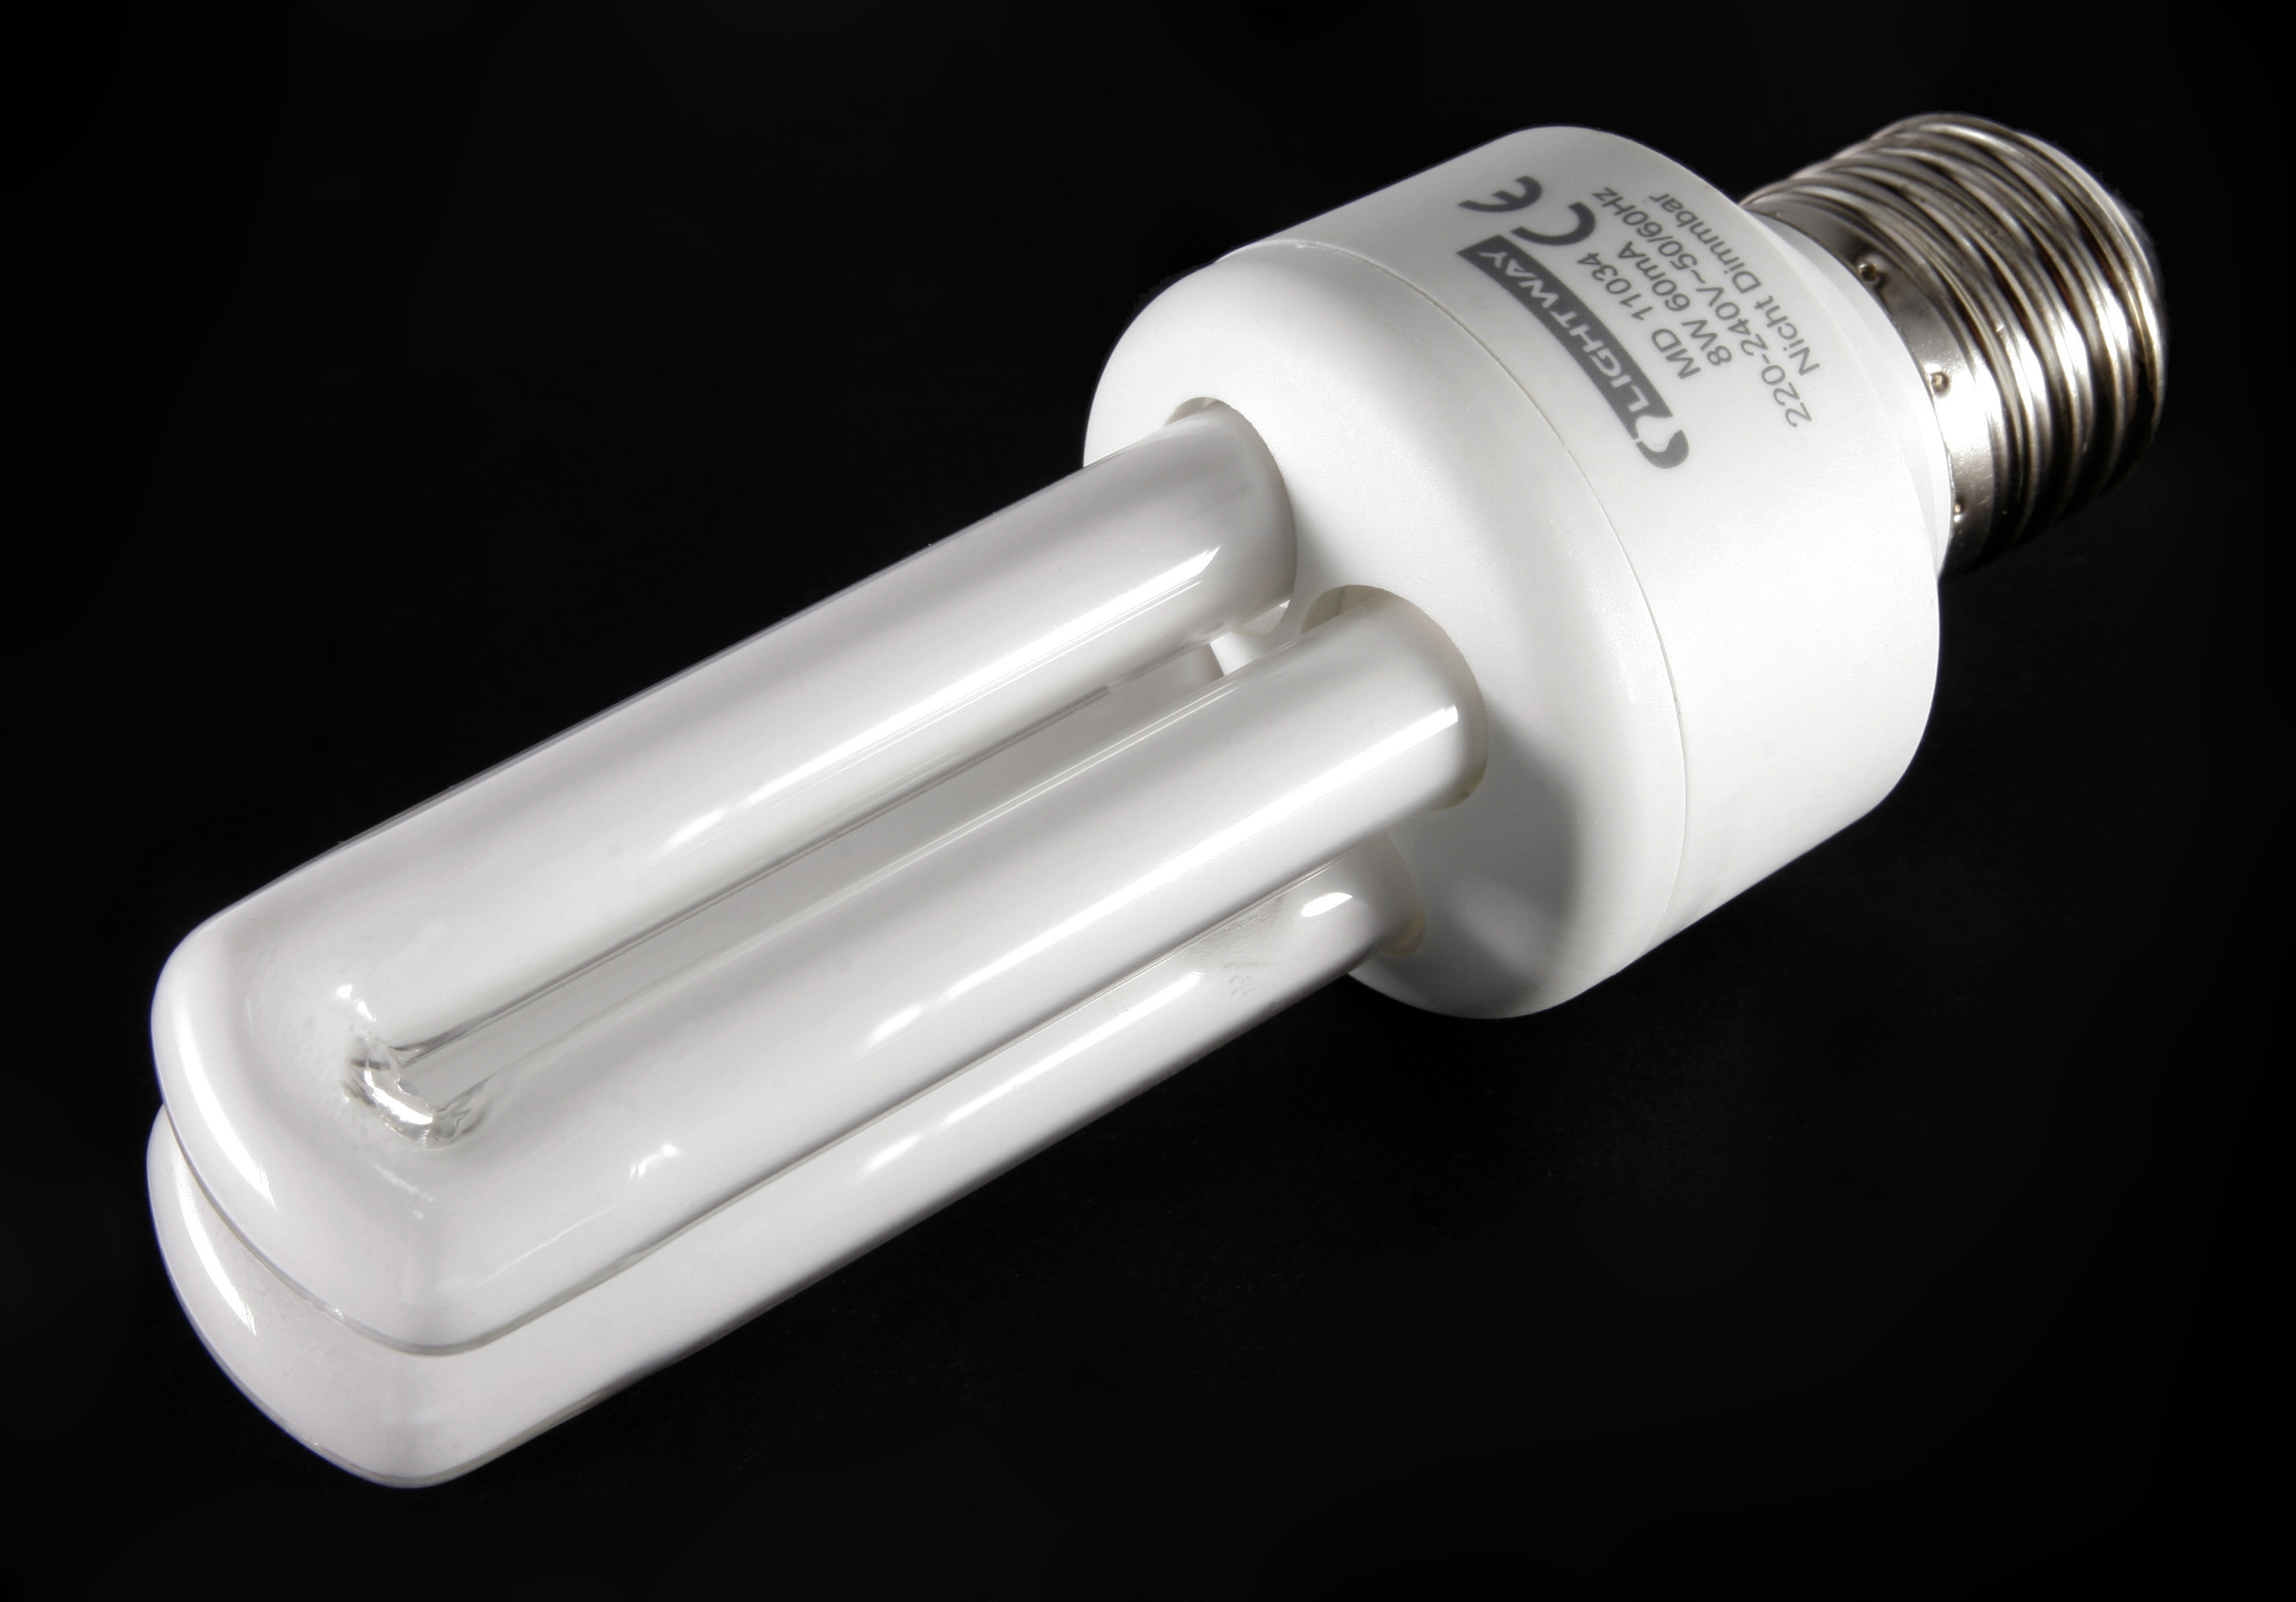
\includegraphics[width=0.5\textwidth]{pictures/bright_light.jpg}
    \caption{Bright Light Source used for paper illumination}
    \label{fig:light}
\end{figure}

A high-intensity compact fluorescent lamp (CFL) is used as the light source, as shown in Figure~\ref{fig:light}. The bright light source is positioned on one side of the paper transport path, directing a uniform beam of light through the paper. A bright and consistent light source is essential to maximise the contrast between normal paper (which absorbs most of the light) and areas with pinholes (which allow the light to pass through). The CFL provides sufficient luminous intensity to ensure reliable LDR response and clear imaging by the ESP32-CAM.

\subsection{ESP32-CAM}

\begin{figure}[H]
    \centering
    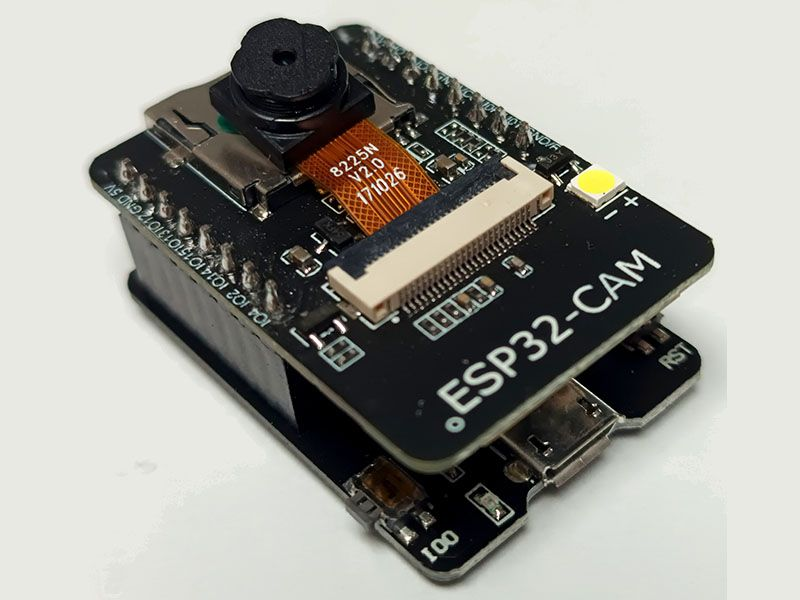
\includegraphics[width=0.5\textwidth]{pictures/esp32_cam.jpg}
    \caption{ESP32-CAM Module}
    \label{fig:espcam}
\end{figure}

The ESP32-CAM, shown in Figure~\ref{fig:espcam}, is a small, low-cost microcontroller module that integrates an ESP32-S chip with an OV2640 camera and built-in Wi-Fi and Bluetooth capabilities. It is capable of capturing images and streaming video over a network.

In this system, the ESP32-CAM is mounted within the detection chamber and oriented to capture images of the paper surface during inspection. When triggered by the ESP32 (upon an LDR anomaly detection), the module captures a still image and transmits it to the host computer software via an HTTP POST request to a dedicated API endpoint. This allows the machine learning model to perform a secondary visual confirmation of detected pinholes.

\subsection{ESP32 Microcontroller}

\begin{figure}[H]
    \centering
    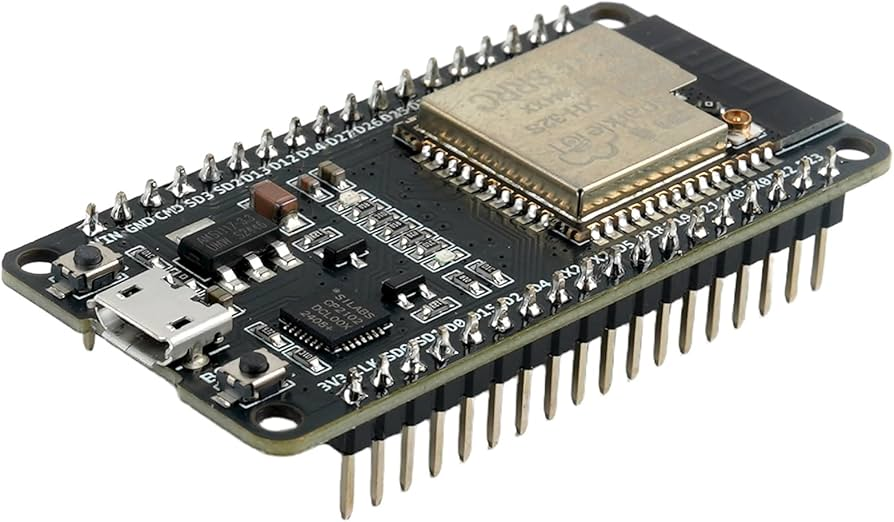
\includegraphics[width=0.5\textwidth]{pictures/esp32.jpg}
    \caption{ESP32 Microcontroller}
    \label{fig:esp32}
\end{figure}

The ESP32, shown in Figure~\ref{fig:esp32}, is a powerful, low-cost, low-power system-on-chip (SoC) microcontroller with integrated Wi-Fi and Bluetooth. It features dual-core processing, numerous GPIO pins, ADC (Analogue-to-Digital Converter) channels, and support for multiple communication protocols including I\textsuperscript{2}C, SPI, UART, and MQTT.

The ESP32 serves as the central controller of the hardware unit. It reads the analogue output from the LDR sensors through its ADC channels, controls the relay module to manage the wiper motor, drives the LCD display to show system status and detection results, and communicates with the host software over Wi-Fi using the MQTT protocol. Upon receiving a detection command or result from the software, the ESP32 can trigger appropriate responses such as stopping the motor or flagging the defective paper section.

\subsection{Wiper Motor}

\begin{figure}[H]
    \centering
    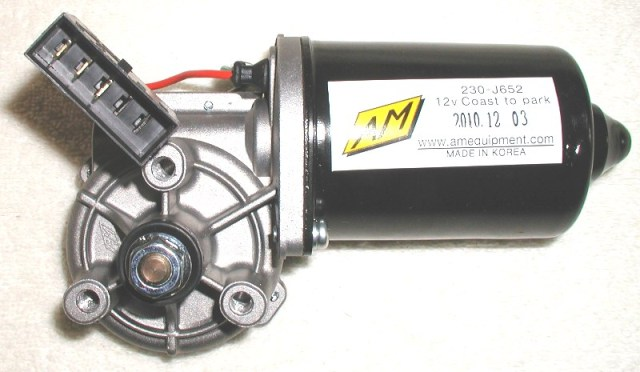
\includegraphics[width=0.5\textwidth]{pictures/wiper_motor.jpg}
    \caption{Automotive Wiper Motor}
    \label{fig:wiper}
\end{figure}

An automotive wiper motor, shown in Figure~\ref{fig:wiper}, is used to drive the paper transport mechanism. Wiper motors are inherently designed to operate at low, consistent speeds — a characteristic that is essential for this application, as the paper must move slowly and uniformly through the detection chamber to allow sufficient time for the LDRs and ESP32-CAM to scan each section accurately.

The primary advantage of selecting a wiper motor over alternatives such as a standard DC motor with a Variable Frequency Drive (VFD) is that the wiper motor naturally operates at a low RPM without requiring additional speed-control circuitry. This simplifies the mechanical design and reduces overall system cost. The motor is powered by the 12V power supply and its operation is controlled via the relay module.

\subsection{Power Supply}

\begin{figure}[H]
    \centering
    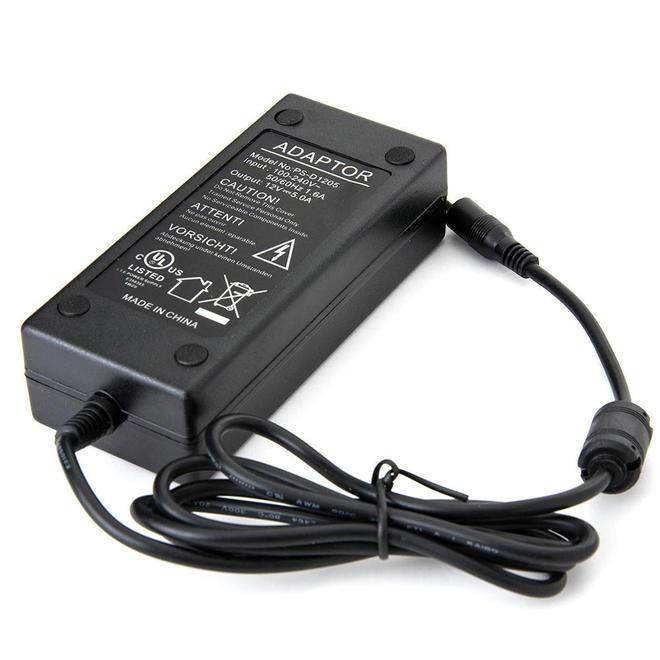
\includegraphics[width=0.5\textwidth]{pictures/power_supply.jpg}
    \caption{12V DC Power Supply}
    \label{fig:psu}
\end{figure}

A 12V DC power supply, shown in Figure~\ref{fig:psu}, provides the primary power for the system. The 12V rail directly powers the wiper motor through the relay module. The same 12V supply also feeds the buck converter, which steps the voltage down to 5V for the ESP32 and other logic-level components. Using a single 12V supply for the entire system simplifies the power distribution architecture and reduces the number of external power adapters required.

\subsection{Relay Module}

\begin{figure}[H]
    \centering
    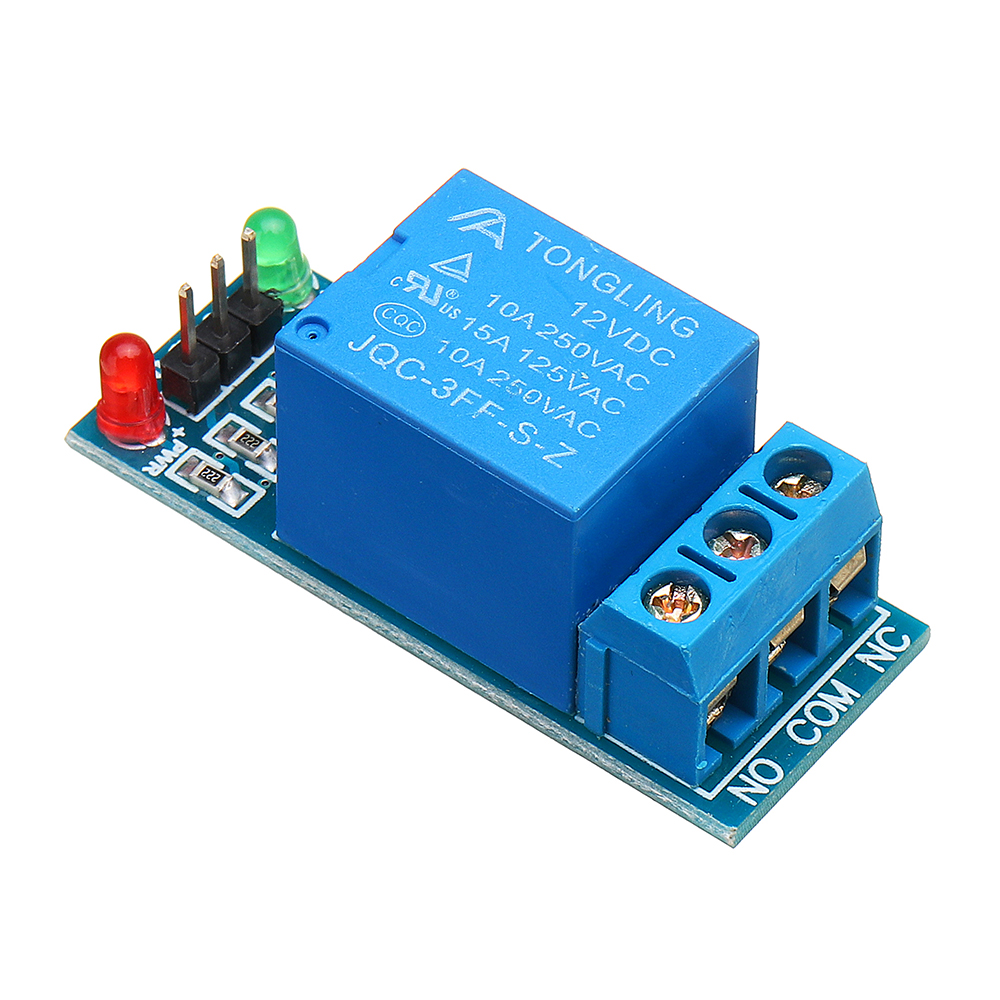
\includegraphics[width=0.5\textwidth]{pictures/relay_module.png}
    \caption{12V Relay Module (5A)}
    \label{fig:relay}
\end{figure}

The relay module, shown in Figure~\ref{fig:relay}, is an electrically operated switch that allows the low-voltage ESP32 to control the high-voltage wiper motor circuit. The relay used is rated at 12V DC with a 5A current capacity, making it suitable for switching the wiper motor load safely.

When the ESP32 asserts a control signal to the relay's input pin, the relay coil is energised, closing the contact and completing the circuit between the 12V supply and the wiper motor. This enables the ESP32 to start and stop the motor as required during the detection process without any direct electrical connection between the microcontroller and the high-current motor circuit, thus protecting the ESP32 from voltage and current damage.

\subsection{\texorpdfstring{LCD 20$\times$4 I\textsuperscript{2}C Display}{LCD 20x4 I2C Display}}

\begin{figure}[H]
    \centering
    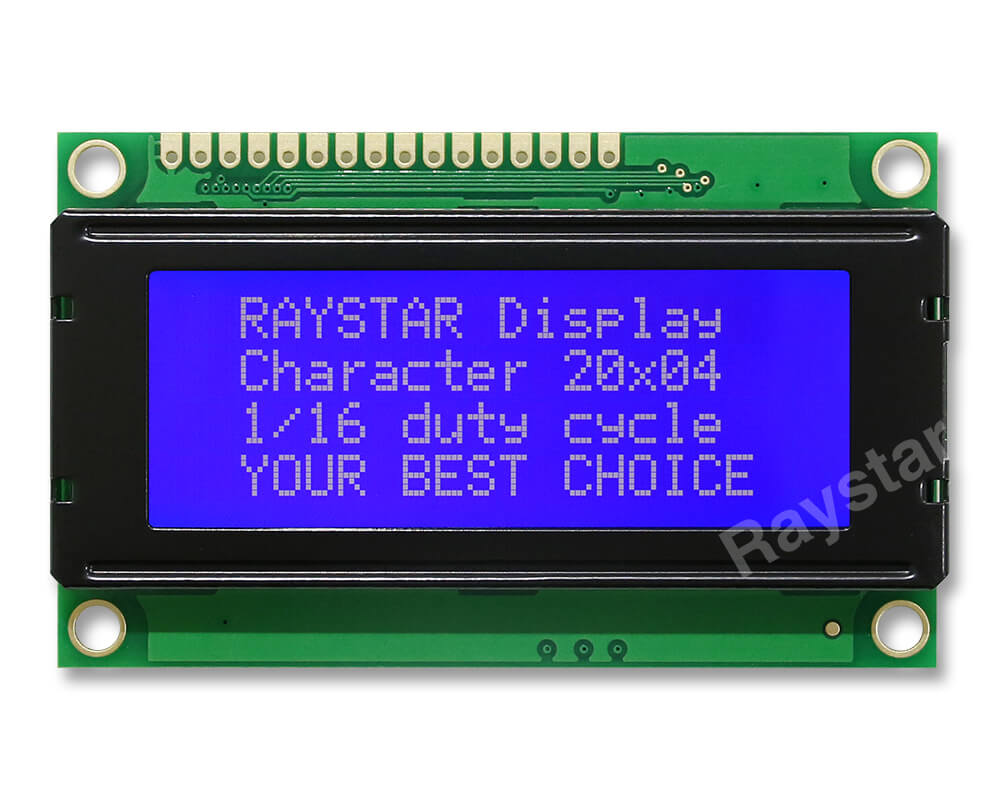
\includegraphics[width=0.55\textwidth]{pictures/lcd.jpg}
    \caption{20$\times$4 Character LCD with I\textsuperscript{2}C Interface}
    \label{fig:lcd}
\end{figure}

The 20$\times$4 character LCD module with I\textsuperscript{2}C interface, shown in Figure~\ref{fig:lcd}, provides a local user interface for the detection system. The display is capable of showing 4 rows of 20 characters each, which is sufficient to present system status messages, detection results, motor state, and Wi-Fi connectivity information.

The I\textsuperscript{2}C interface requires only two signal lines (SDA and SCL) to communicate with the ESP32, minimising the number of GPIO pins used. This is particularly advantageous given that the ESP32 must also manage the LDR ADC channels, relay control, and MQTT communication simultaneously.

\subsection{Buck Converter}

\begin{figure}[H]
    \centering
    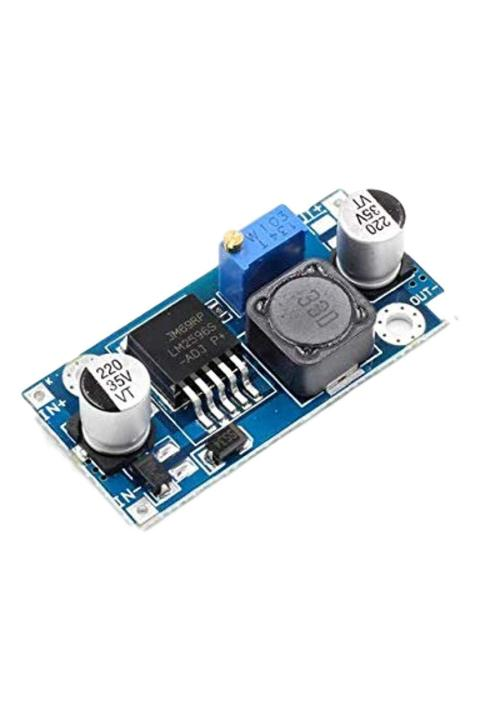
\includegraphics[width=0.45\textwidth]{pictures/buck_coverter.jpg}
    \caption{DC-DC Buck Converter (12V to 5V)}
    \label{fig:buck}
\end{figure}

A DC-DC buck converter, shown in Figure~\ref{fig:buck}, is a step-down voltage regulator that efficiently converts the 12V supply voltage to the 5V required by the ESP32 microcontroller and other logic-level components. Unlike linear regulators, a buck converter achieves voltage step-down with high efficiency (typically above 85\%), generating significantly less heat and wasting less power, which is important for a continuously running embedded system.

The buck converter takes the 12V input from the primary power supply and outputs a regulated 5V to power the ESP32, LCD module, and relay control circuitry, ensuring stable operation of all electronic components throughout the detection process.

\section{Software Design}

The software subsystem is responsible for receiving images from the ESP32-CAM, classifying them using a trained machine learning model, and returning detection results to the hardware via MQTT. The software runs on a host computer connected to the same Wi-Fi network as the ESP32 and ESP32-CAM.

\subsection{Flask Web Server and API}

The software is built using Flask, a lightweight Python web framework. Flask exposes a RESTful HTTP API with a dedicated endpoint to which the ESP32-CAM sends captured images. Upon receiving an image via an HTTP POST request to the API route, the server immediately passes the image to the machine learning inference module for processing. Flask was selected for its simplicity, minimal overhead, and ease of integration with Python-based machine learning libraries.

\subsection{Machine Learning Model}

A machine learning model is trained using Python to classify captured images as either containing a pinhole or being defect-free. The model is trained on a labelled dataset of paper images, learning the visual signatures associated with pinholes under the system's lighting conditions. Once trained, the model is serialised and loaded by the Flask application at startup, ready for real-time inference on incoming images from the ESP32-CAM.

\subsection{MQTT Communication}

The Message Queuing Telemetry Transport (MQTT) protocol is used for communication from the software back to the ESP32 hardware. After the machine learning model produces a classification result, the Flask server publishes the result as an MQTT message to a broker. The ESP32, subscribed to the relevant MQTT topic, receives the message and takes the appropriate action, such as stopping the wiper motor or displaying an alert on the LCD. MQTT was chosen for its low bandwidth usage, low latency, and suitability for embedded IoT applications.

\section{Mechanical Design}

The mechanical structure of the detection system was designed using SolidWorks, a professional 3D computer-aided design (CAD) software package. The design encapsulates the paper transport mechanism, the light source housing, the LDR mounting array, the camera mount, and the electronics enclosure into a single integrated unit.

The wiper motor is mechanically coupled to a roller mechanism that drives the banknote paper through the detection chamber at a controlled, low speed. The light source is positioned on one side of the paper path within a sealed housing to prevent ambient light from interfering with LDR readings. The LDR array is mounted directly opposite the light source on a fixed bracket to maintain consistent sensor-to-paper distance during operation.

The SolidWorks model allowed for precise dimensioning and assembly verification before physical fabrication, reducing the risk of component fit issues and ensuring that the optical alignment between the light source, paper, and LDR sensors was maintained accurately throughout operation.
